\documentclass{article}
\usepackage{tikz}

\begin{document}

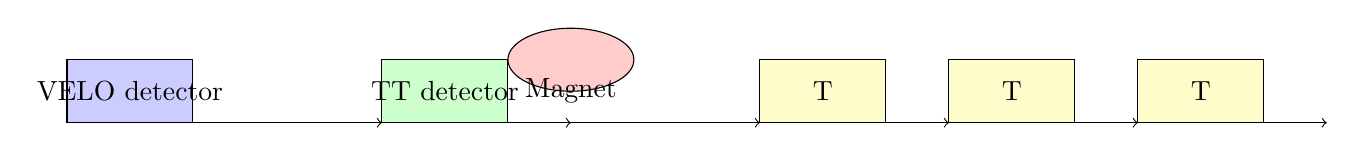
\begin{tikzpicture}[scale=0.8]
    % Draw the VELO detector
    \draw[fill=blue!20] (-5,0) rectangle (-3,-1);
    \node at (-4,-0.5) {VELO detector};

    % Draw the TT detector
    \draw[fill=green!20] (0,0) rectangle (2,-1);
    \node at (1,-0.5) {TT detector};

    % Draw the Magnet
    \draw[fill=red!20] (3,0) ellipse (1 and 0.5);
    \node at (3,-0.5) {Magnet};

    % Draw the Downstream Tracking Stations
    \draw[fill=yellow!20] (6,0) rectangle (8,-1);
    \node at (7,-0.5) {T};
    \draw[fill=yellow!20] (9,0) rectangle (11,-1);
    \node at (10,-0.5) {T};
    \draw[fill=yellow!20] (12,0) rectangle (14,-1);
    \node at (13,-0.5) {T};

    % Connect the components
    \draw[->] (-4,-1) -- (0,-1);
    \draw[->] (0,-1) -- (3,-1);
    \draw[->] (3,-1) -- (6,-1);
    \draw[->] (6,-1) -- (9,-1);
    \draw[->] (9,-1) -- (12,-1);
    \draw[->] (12,-1) -- (15,-1);

\end{tikzpicture}

\end{document}